\documentclass[a4paper, 12pt]{article}
\usepackage[top=2cm, bottom=2cm, left=2.5cm, right=2.5cm]{geometry}
\usepackage[utf8]{inputenc}
\usepackage[brazilian]{babel}
\usepackage{indentfirst}
\usepackage{graphicx}
\usepackage{wrapfig}
\usepackage[pdftex]{hyperref}
\graphicspath{ {imagens/} }
\usepackage{amsmath}

\begin{document}
%
\begin{titlepage} %iniciando a "capa"
	\begin{center} %centralizar o texto abaixo
		{\large Unicamp}\\[0.4cm] %0,2cm é a distância entre o texto dessa linha e o texto da próxima
		{\large Professor João Batista Fogagnolo}\\
		{\large ES365A}\\[3.2cm]
		{\bf \huge Trabalho Fabricação Mecânica e Metalúrgica}\\[0.2cm] 
		{\bf \large Fundição}\\[4.9cm]
		% o comando \bf deixa o texto entre chaves em negrito. O comando \huge deixa o texto enorme
	\end{center} %término do comando centralizar
	{\large Erik Yuji Goto}\\ % o comando \large deixa o texto grande
	RA: 234009\\[10cm]
	\begin{center}
	
		{\large Campinas}\\[0.2cm]
		{\large 2022}
	\end{center}
\end{titlepage} %término da "capa"


\tableofcontents
\newpage

\section{O que é fundição?}
	O processo de fundição consiste em produzir uma peça a partir do metal fundido, em estado líquido. O material é derramado em um molde e após solidificado fica com a geometria interna do molde.
	Comparando com outros processos de fabricação, o processo de fundição é mais vantajoso nos seguintes aspectos:
	\begin{itemize}
		\item Complexidade de formas que podem ser produzidas;
		\item Ampla gama de materiais que após solidificados assumem a geometria do modelo;
			\begin{itemize}
				\item Uma propriedade importante da liga metálica a ser utilizada é sua fluidez. O material deve preencher todos os espaços livres do molde. Uma liga muito visgosa pode dificultar o preenchimento interno do molde, e como resultado teremos muitas imperfeições na peça final.
			\end{itemize}
		\item Ampla gama de propriedades que podem ser controladas durante o processo;
		\item Usado para pequenos ou elevadas quantidades de peças;
		\item Baixo custo, pois não utiliza de ferramentas e materiais muito caros;
		\item Elevada precisão dimensional e acabamento;
		\item \textit{Near net shape} em uma única operação, ou seja, após sair da fundição a peça tem uma geometria próxima da peça final, sendo necessário apenas alguns processos para acabamento. 
	\end{itemize}

	O processo de fundição é dividido em dois grandes grupos: fundição em moldes colapsáveis e em moldes permanentes.
	
	Em processos de fundição em moldes colapsáveis o molde só é usado uma vez, pois ele é desmontado para a retirada da peça pronta, além disso o material do molde pode ser reutilizado para a produção de mais peças. São exemplos: moldes de areia, shell molding, fundição com cera perdida.
	
	Já os moldes permanentes podem ser usados mais de uma vez, sem a necessidade de destruir o molde e é restrito a peças de pequenas dimensões. Exemplos: por gravidade, por compressão.

	\subsection{Canais de alimentação e Massalotes}
	Dois conceitos básicos para entender melhor a fundição são os canais de alimentação e massalotes. 
	
	Os canais de alimentação são dutos que conduzem a liga metálica no estado líquido para o interior do molde.
	
	O resfriamento da peça após o depósito de metal no molde acontece de fora para dentro, sendo que a camada em contato com o molde perde mais calor. Este fenômeno, junto com a dilatação térmica, faz com que a peça precise de mais metal para compensar a diminuição de sua dimensão. Os massalotes são reservatórios que tem função de resolver esse problema, ao suprir a peça com mais metal, com isso evitamos que o interior da peça fique com vazios após a solidificação do material.
	\begin{figure}[h]
			\centering
			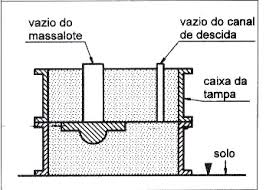
\includegraphics[scale=0.5]{a.jpeg}
			\caption{Canal de Alimentação e Massalote}
		\end{figure}
	\section{Fundição em Areia verde}
	Este tipo de fundição é o mais utilizado devido a sua versatilidade. Para ilustrar o processo de fundição foi utilizada imagens de um video da internet\footnote{Casting Kirito´s Elucidator (Sword Art Online) - AlumiTube: https://youtu.be/1y2FFdHzloQ}
	\begin{enumerate}
		\item O modelo é colocado no fundo da caixa que será feita a fundição, e em cima dele é depositado talco ou grafite para facilitar sua posterior retirada;
		\begin{figure}[h]
			\centering
			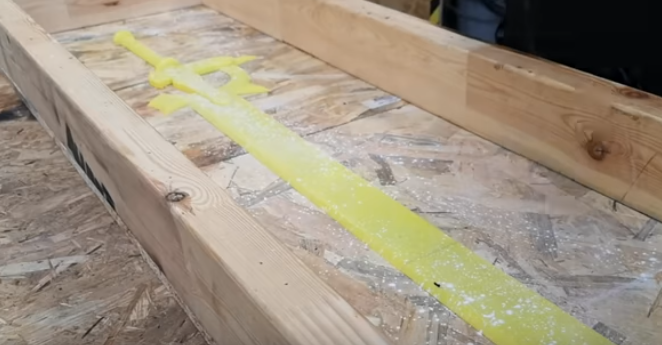
\includegraphics[scale=0.5]{a.png}
			\caption{Modelo coberto com talco}
		\end{figure}
		\item A areia é depositada em cima do modelo até preencher a caixa e pressionada para evitar poros grandes. Note que, o molde de areia precisa ser resistente o suficiente para manter sua geometria antes e durante o processo de injeção de metal líquido;
		\begin{figure}[h]
			\centering
			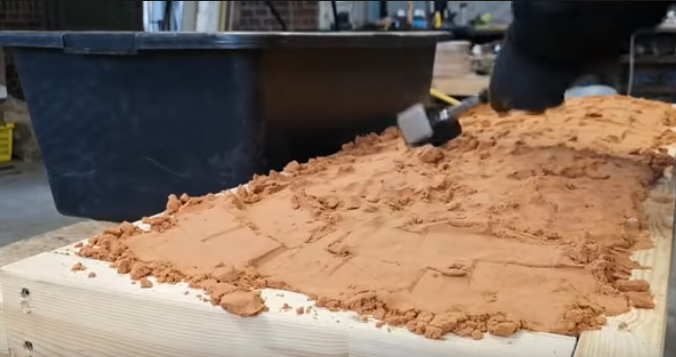
\includegraphics[scale=0.5]{a1.png}
			\caption{Modelo coberto com areia}
		\end{figure}
		\item A caixa é virada de ponta cabeça para que o modelo fique virado para cima. É adicionado a caixa-tampa, e nela os massalotes e canais de alimentação(em vermelho);
		\item Novamente é adicionado areia na caixa-tampa e ela é compactada;
		\item O próximo passo é retirar os massalotes e canais de alimentação;
		\begin{figure}[h]
			\centering
			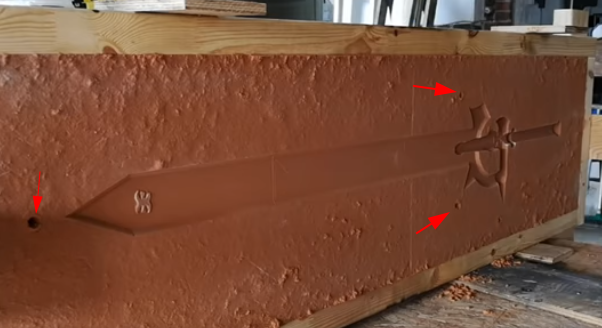
\includegraphics[scale=0.5]{a2.png}
			\caption{Tampa da caixa apenas com os canais de alimentação}
		\end{figure}
		\item Na caixa-fundo o modelo é retirado, e é feita um canal de entrada ligando o canal de alimentação com o local onde o modelo estava;
		\item O conjunto de caixas é montado novamente e as caixas são fixadas com presilhas ou grampos, com isso temos o molde pronto para a fundição;
		\item Basta derramar o metal líquido pelo canal de alimentação, esperar resfriar e fazer a desmontagem. Após a desmontagem do molde até 98\% da areia pode ser reutilizada.
		\begin{figure}[h]
			\centering
			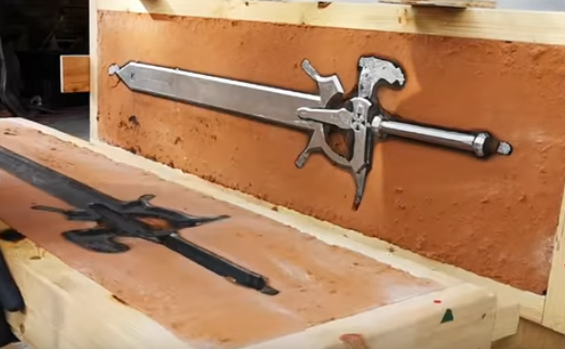
\includegraphics[scale=0.5]{a3.png}
			\caption{Retirada da peça fundida}
		\end{figure}
		\item A peça precisa passar por alguns processos de usinagem, como a retirada do excesso de material dos canais de alimentação, e um acabamento para alcançar sua geometria final. 
		\begin{figure}[h]
			\centering
			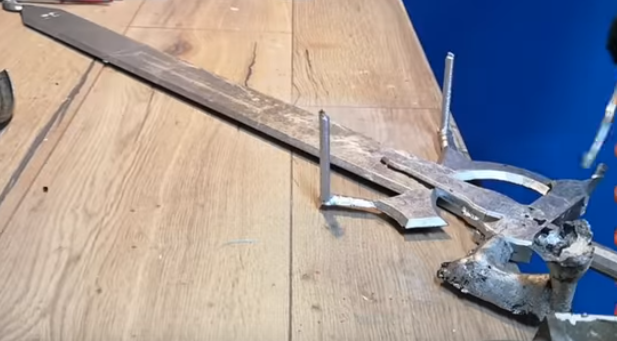
\includegraphics[scale=0.5]{a4.png}
			\caption{Peça pronta para ser usinada}
		\end{figure}
	\end{enumerate}
	
	\newpage
	\section{Fundição com Cera Perdida}
		O processo de fundição de precisão, ou cera perdida, usa cera como modelo, e é envolto de cerâmica para formar o molde após endurecido. Para retirar o molde é necessário derreter a cera, destruindo assim o modelo. Depois que a liga metálica é solidificada o molde de cerâmica é então colapsado. Portanto, tanto o molde quanto o modelo são destruídos no processo de fundição de precisão.
		
		O processo de fundição com cera perdida é descrita detalhadamente abaixo:
	\begin{enumerate}
	\item Preparação para a fundição: O primeiro passo da fundição com Cera Perdida é produzir o molde.
		\begin{enumerate}
			\item Inicialmente o modelo é feito com uma cera especial utilizando um molde metálico;
				\begin{figure}[h]
					\centering
					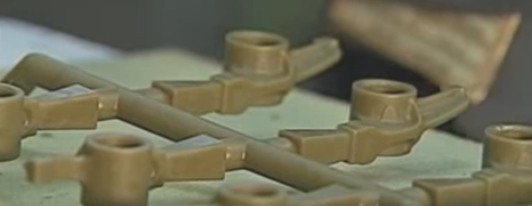
\includegraphics[scale=0.5]{a5.png}
					\caption{Modelo de cera}
				\end{figure}
			\item Com vários modelos já prontos, eles são alocados em cachos. Nos mesmos cachos são adicionados os canais de alimentação e vazamento necessários para garantir uma fundição de qualidade;
				\begin{figure}[h]
					\centering
					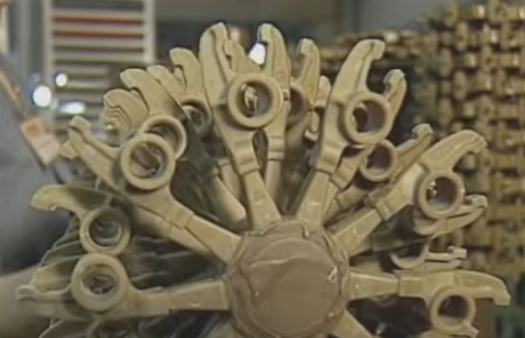
\includegraphics[scale=0.5]{a6.png}
					\caption{Cachos com os canais de alimentação}
				\end{figure}
			\item O cacho é submerso em uma solução de cerâmica contendo ligantes. Dessa forma, é criada uma casca em volta das peças. Após isso, adiciona-se uma camada de partículas refratárias contendo zirconita, silimita e alumínio-silicato;
				\begin{figure}[h]
					\centering
					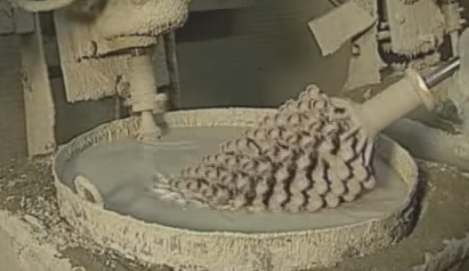
\includegraphics[scale=0.5]{a7.png}
					\caption{Cacho submerso na solução cerâmica}
				\end{figure}
			\item Espera-se a secagem da casca, e então o modelo de cera é derretido para produzir um molde oco;
			\item Para endurecer o molde cerâmico, ele é sinterizado entre 650ºC e 1000ºC. 	
		\end{enumerate}
	\item Injeção do Metal
		\begin{enumerate}
			\item Após o endurecimento do molde podemos adicionar o metal líquido;
				\begin{figure}[h]
					\centering
					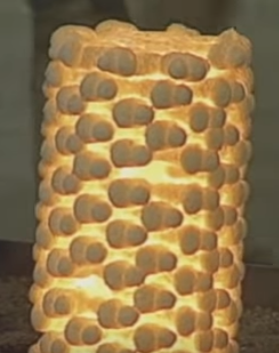
\includegraphics[scale=0.5]{a8.png}
					\caption{Molde após ser adicionado o metal líquido}
				\end{figure}
			\item Com a solidificação final do metal a casca cerâmica é colapsada e conseguimos ter acesso às peças finais;
			\item O último passo é realizar as usinagens e processos de acabamento necessários para ter uma peça com as dimensões finais de projeto.
		\end{enumerate}
	\end{enumerate}
	
	\section{Fundição sob Pressão}
	Na fundição sob pressão, a liga metálica é pressionada sob baixa pressão e baixa velocidade para o interior da cavidade do molde permanente. Este tipo de fundição é aplicado principalmente para ligas de alumínio, pois possuem menos viscosidade portanto necessitam de menores pressões para preencher completamente o molde.
	
	Vantagens:	
	\begin{itemize}
		\item Não solidifica canais, portanto dispensa operações de corte;
		\item Fundido livre de poros e óxidos;
	\end{itemize}
	Desvantagens:
	\begin{itemize}
		\item Pressões baixas podem causar mal acabamento e outros defeitos de preenchimento;
		\item Não é possível produzir peças muito grandes.
	\end{itemize}
	
	As etapas da fundição sob pressão são:
	\begin{enumerate}
		\item Em cima da panela contendo o metal é posto o molde e fechado por pressão hidráulica(I/II);
		\item É aplicada uma pressão tal que o líquido na panela comece a subir e preencher o molde(III);
		\item Essa pressão é mantida até que ocorra a solidificação no interior do molde, quando a pressão é aliviada acontece o refluxo do líquido não solidificado e o mesmo retorna para a panela(IV);
		\item Após isso, pode ser feito os processos de acabamento na peça.
	\end{enumerate}
	
	\begin{figure}[h]
		\centering
		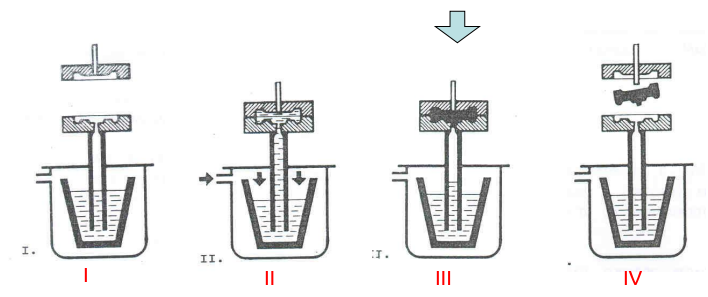
\includegraphics[scale=0.5]{9.png}
		\caption{Processo de Fundição sob pressão}
	\end{figure}
	
	
	
\newpage
\section{Referências Bibliográficas}
	Notas de Aula ES365, professor Joao Batista Fogagnolo, 2022.\\
	
	TÂMEGA, Fábio. Fundição de Processos Siderúrgicos. UFPR, Londrina 2017. \\Disponível em:$<http://ftp.demec.ufpr.br/disciplinas/\\$ $TM233/Arquivos\%20FTP\%202020/Bibliografia/LIVRO_processo_de_fundicao.pdf>$\\

	TELECURSO 2000. Curso Profissionalizante Mecânica - Processos de Fabricação(Teleaula 04)
\end{document}

	